\chapter{Implementacija i korisničko sučelje}
		
		
		\section{Korištene tehnologije i alati}
		
			Komunikacija u timu odvijala se videopozivima putem aplikacije \underline{\href{https://www.microsoft.com/en-us/microsoft-teams/group-chat-software}{Microsoft Teams}}\textsuperscript{1}. Za izradu UML dijagrama korišteni su alati \underline{\href{https://astah.net/products/astah-uml/}{Astah UML}}\textsuperscript{2} i \underline{\href{https://online.visual-paradigm.com/}{Visual Paradigm}}\textsuperscript{3}. \underline{\href{https://git-scm.com/}{Git}}\textsuperscript{4} je korišten kao sustav za upravljanje kodom. Projekt je dostupan na web platformi \underline{\href{https://github.com/}{GitHub}}\textsuperscript{5}
			
			\indent Za razvoj aplikacije korištena su razvojna okruženja \underline{\href{https://www.jetbrains.com/idea/}{IntelliJ IDE}}\textsuperscript{6} i \newline\underline{\href{https://code.visualstudio.com/}{Visual Studio Code}}\textsuperscript{7}. IntelliJ jedan je od najpopularnijih razvojnih okruženja za razvoj aplikacija u programskom jeziku Java. Izgradila ga je tvrtka JetBrains. Pruža bogatu podršku za razvoj desktop i web aplikacija. Visual Studio Code je također vrlo popularan uređivač za pisanje programskog koda, osobita za razvoj frontend dijela aplikacija jer pruža izrazito dobru podršku za frontend radne okvire. On je pod vlasništvom tvrtke Microsoft.
			
			\indent Aplikacija je napisana koristeći radni okvir \underline{\href{https://spring.io/projects/spring-boot/}{Spring Boot}}\textsuperscript{8} i jezik \underline{\href{https://www.oracle.com/java/}{Java}}\textsuperscript{9} za izradu \textit{backenda} te \underline{\href{https://react.dev/}{React}}\textsuperscript{10} i jezik \underline{\href{https://www.javascript.com/}{JavaScript}}\textsuperscript{11} za izradu \textit{frontenda}. React je biblioteka izražena u JavaScriptu koja olakšava izradu korisničkog sučelja. React je održava tvrtka Meta. Radni okvir Spring Boot nadograđuje mogućnosti samog programskog jezika Java te time uvelike olakšava razvoj web aplikacija. Nudi niz gotovih funkcionalnosti koji povećavaju produktivnost i efikasnost programera.
			
			\indent Za bazu podataka korišten je \underline{\href{https://www.postgresql.org/}{PostgreSQL}}\textsuperscript{12}.
			\noindent\\[1ex]\rule{0.5\linewidth}{0.5pt}\newline
			\noindent\textsuperscript{1}\url{https://www.microsoft.com/en-us/microsoft-teams/group-chat-software}\newline
			\noindent\textsuperscript{2}\url{https://astah.net/products/astah-uml/}\newline
			\noindent\textsuperscript{3}\url{https://online.visual-paradigm.com/}\newline
			\noindent\textsuperscript{4}\url{https://git-scm.com/}\newline
			\noindent\textsuperscript{5}\url{https://github.com/}\newline
			\noindent\textsuperscript{6}\url{https://www.jetbrains.com/idea/}\newline
			\noindent\textsuperscript{7}\url{https://code.visualstudio.com/}\newline
			\noindent\textsuperscript{8}\url{https://spring.io/projects/spring-boot/}\newline
			\noindent\textsuperscript{9}\url{https://www.oracle.com/java/}\newline
			\noindent\textsuperscript{10}\url{https://react.dev/}\newline
			\noindent\textsuperscript{11}\url{https://www.javascript.com/}\newline
			\noindent\textsuperscript{12}\url{https://www.postgresql.org/}\newline
			
		\newpage
		
		\section{Ispitivanje programskog rješenja}
			
			\indent Za provođenje testiranja naše Spring Boot aplikacije koristili smo biblioteke JUnit i Mockito. One su nam omogućile pouzdano i sustavno testiranje različitih dijelova aplikacije. Za ispitivanje sustava koristili smo alat Selenium.
			 
	
			
			\subsection{Ispitivanje komponenti}
			U nastavku ovog poglavlja, pronaći ćete detaljan opis šest odabranih ispitnih slučajeva koji obuhvaćaju redovne situacije, rubne uvjete te testiranje ponašanja sustava u situacijama iznimki. Uz opis ispitnih slučajeva, priložili smo i odgovarajući izvorni kôd svakog testa, kao i rezultate izvođenja ispita u razvojnom okruženju, što omogućuje transparentnost i preglednost provedenih ispitivanja.
			
			Prvi test koji smo odradili je dohvaćanje romobila preko njegovog identifikatora. U ovom smo testu testirali servisni sloj naše aplikacije te set test uredno proveo.
			\begin{figure}[h]
				\centering
				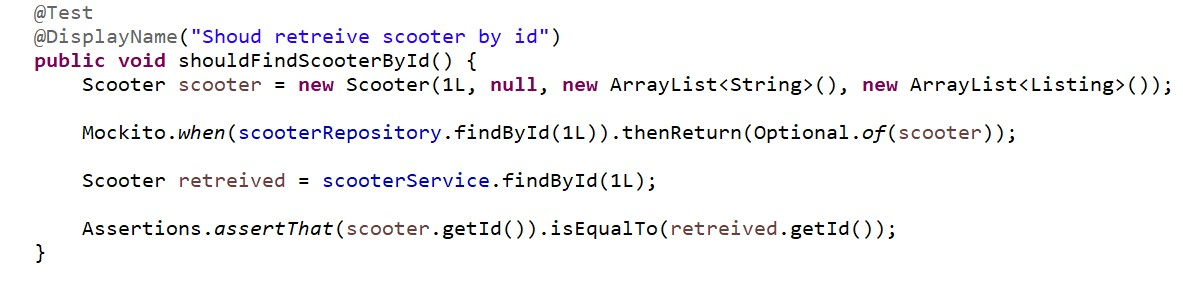
\includegraphics[width=0.6\textwidth]{slike/scooter_service_test.jpg}
				\caption{Testiranje dohvaćanja romobila preko identifikatora}
				\label{fig:Testiranje dohvaćanja romobila preko identifikatora}
			\end{figure}
			
			U sljedećem testu također smo testirali servisni sloj i to dohvaćanje poruka za dva korisnika. Dakle, u testu definiramo dva korisnika te provjeravamo vraća li nam naša aplikacija tražene poruke.
			\begin{figure}[h]
				\centering
				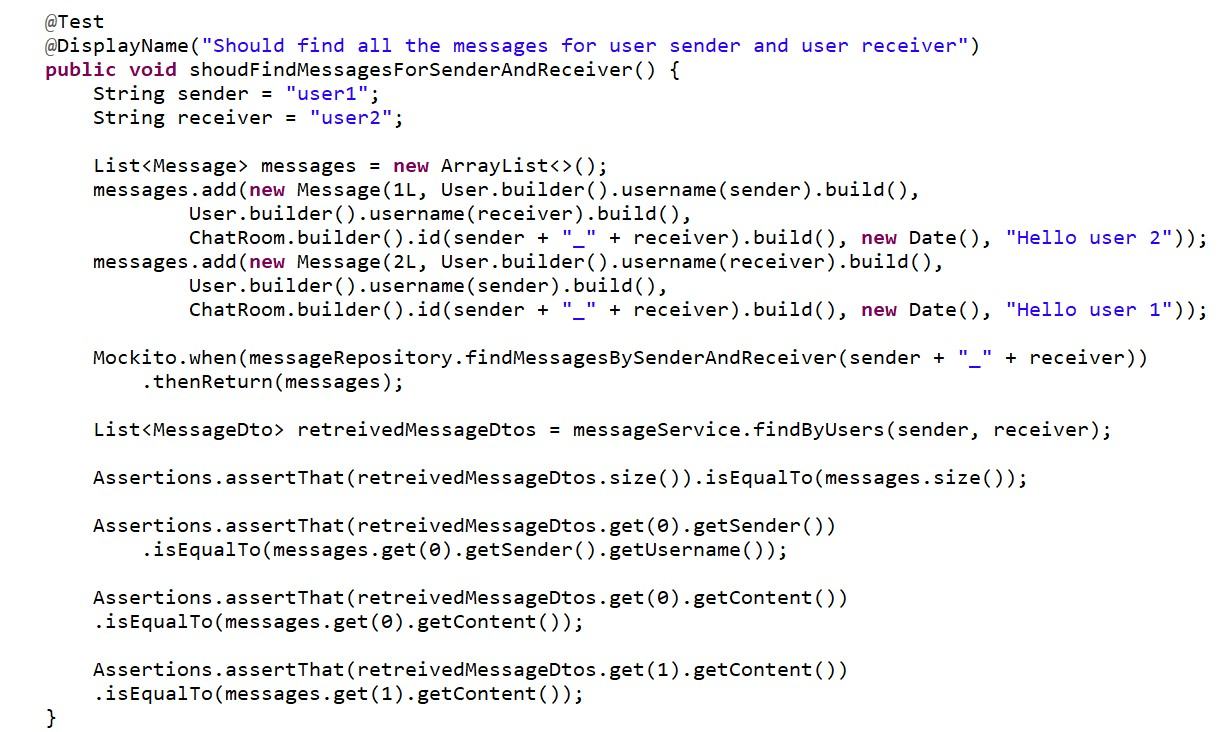
\includegraphics[width=0.6\textwidth]{slike/message_service_test.jpg}
				\caption{Testiranje dohvaćanja poruka za zadane korisnike}
				\label{fig:Testiranje dohvaćanja poruka za zadane korisnike}
			\end{figure}
			
			Sada ćemo prikazati testiranje ListingController. U prvom testu testirali smo dodavanje novog oglasa te je očekivani ishod odgovor poslužitelja s novim oglasom, dok smo u drugom pokušali dohvatit oglas za nepostojeći romobil. U drugom testu očekujemo da poslužitelj baci novu NullPointerException iznimku. Oba testa su se izvršila ispravno. \newline
			
			  \begin{figure}
					  	\centering
					  	\subfigure{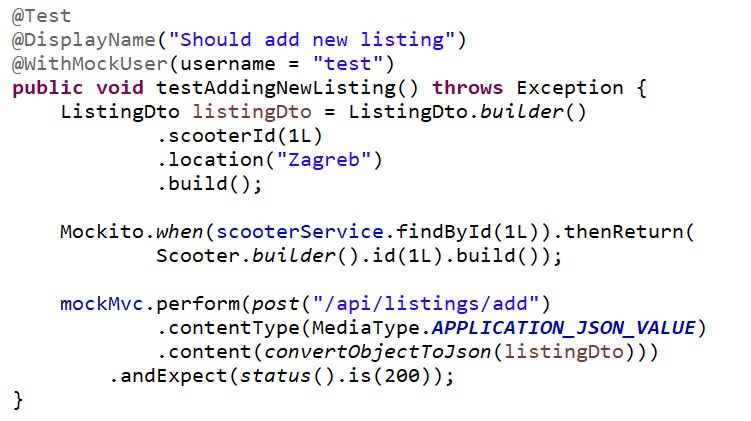
\includegraphics[width=0.4\textwidth]{slike/listing_controller_add_test.jpg}} 
					  	\subfigure{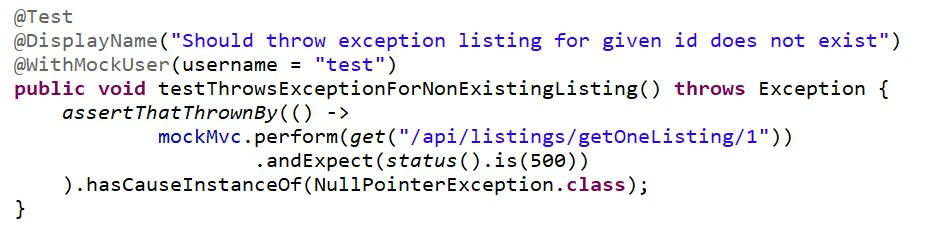
\includegraphics[width=0.4\textwidth]{slike/listing_controller_throw_test.jpg}} 
					  	\caption{Testiranje ListingController-a}
					  	\label{fig:Testiranje ListingController-a}
			  \end{figure}
			  
			Korisnik mora moći pregledavati romobile koje je trenutno iznajmio pa smo testirali i RentalController i to metodu koja osigurava dohvaćanje trenutnih najmova. U testu definiramo koje objekte tipa Rental očekujemo te kada primimo odgovor od poslužitelja provjeravamo jesmo li ih uistinu i primili. \newline
			
			\begin{figure}[h]
				\centering
				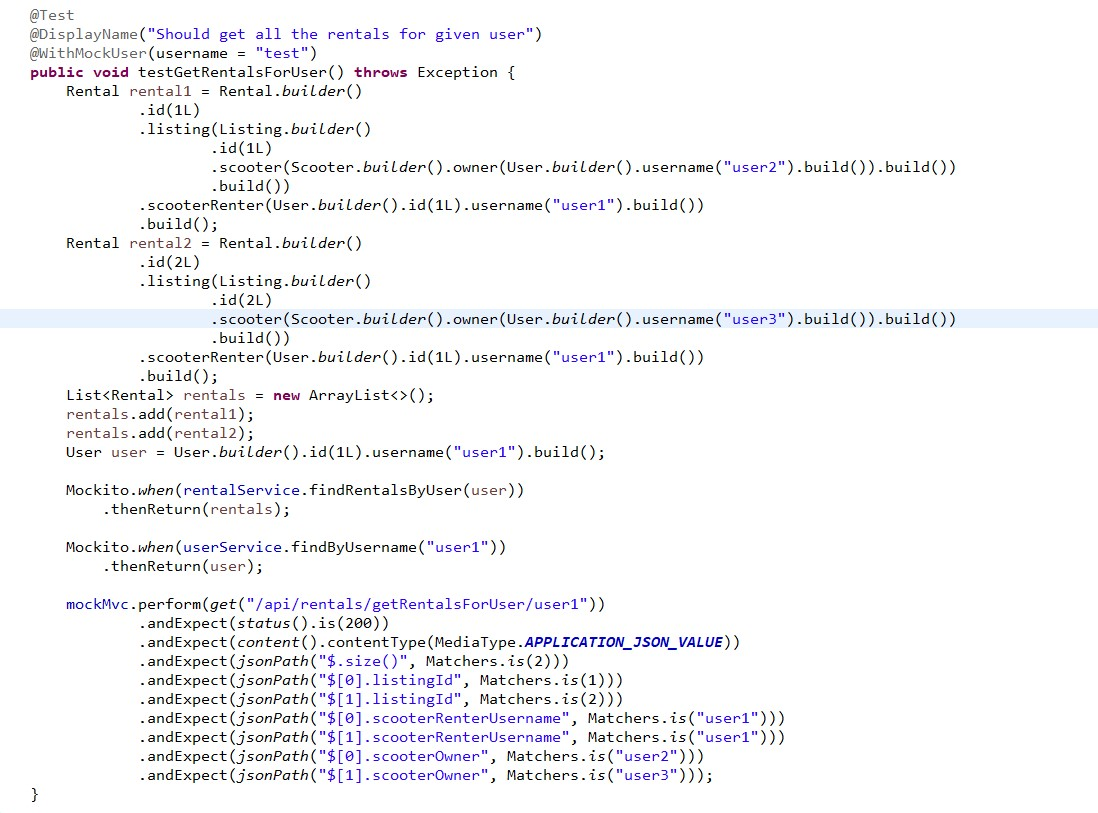
\includegraphics[width=0.6\textwidth]{slike/rental_controller_test.jpg}
				\caption{Testiranje dohvaćanja najmova za korisnika}
				\label{fig:Testiranje dohvaćanja najmova za korisnika}
			\end{figure}
			
			Na kraju, provjerili smo što će se dogodit ako pokušamo izbrisat ocjenu i komentar. Poslužitelj je prepoznao da ta funkcionalnost nije implementirana te ispravno odgovorio sa statusom 404 Not found.\newline
			
			\begin{figure}[h]
				\centering
				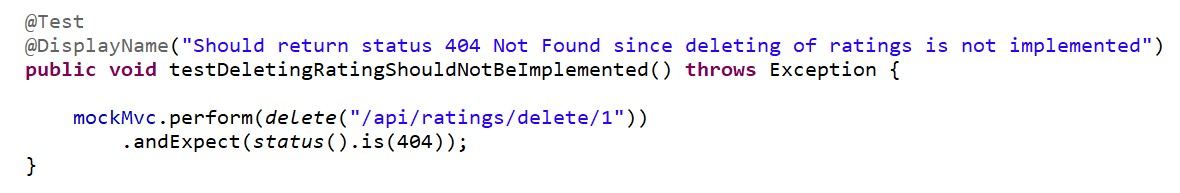
\includegraphics[width=0.6\textwidth]{slike/rating_controller_test.jpg}
				\caption{Testiranje brisanja komentara i ocjena}
				\label{fig:Testiranje brisanja komentara i ocjena}
			\end{figure}
			
			Sljedeća slika prikazuje da su se svi testovi uspješno proveli.
			\begin{figure}[h]
				\centering
				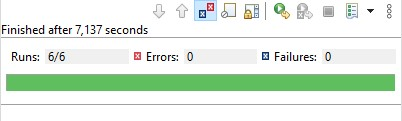
\includegraphics[width=0.6\textwidth]{slike/tests_passed.jpg}
				\caption{Uspješno provođenje testova}
				\label{fig:Uspješno provođenje testova}
			\end{figure}
			
			\subsection{Ispitivanje sustava}
			
			 Za ispitivanje sustava koristili smo alat Selenium WebDriver. Kako bi ga mogli koristit u projekt smo dodali  dependency za Selenium WebDriver. Također, bilo je potrebno i instalirati Chrome WebDriver.\newline
			 
			 \indent U prvom testu testirali smo dvije funkcionalnosti: dodavanje novog romobila i dodavanje oglasa za taj romobil. Korisnik se prvo prijavi u aplikaciju. S obzirom na to da su svi testovi započinjali s prijavom korisnika u aplikaciju, prijavu smo izdvojili u zasebnu funkciju. Koristeći objekt tipa WebDriver provjerili smo je li se korisnik uspješno prijavio u sustav te ako je, pozicionirali smo se na stranicu za pregled romobila. Da bi dodali novi romobil, bilo je potrebno unijeti sliku romobila i to smo učinili metodom sendKeys koju nudi WebDriver. Kliknuli smo na gumb za dodavanje romobila te provjerili je li se romobil uspješno dodao. Zatim smo kliknuli na gumb za dodavanje oglasa, ponovo metodom sendKeys unijeli sve zahtijevane informacije za dodavanje oglasa, dodali oglas i na kraju provjerili je li se oglas uspješno dodao. 
			 
			 \newpage
			 
			 \begin{figure}[h]
			 	\centering
			 	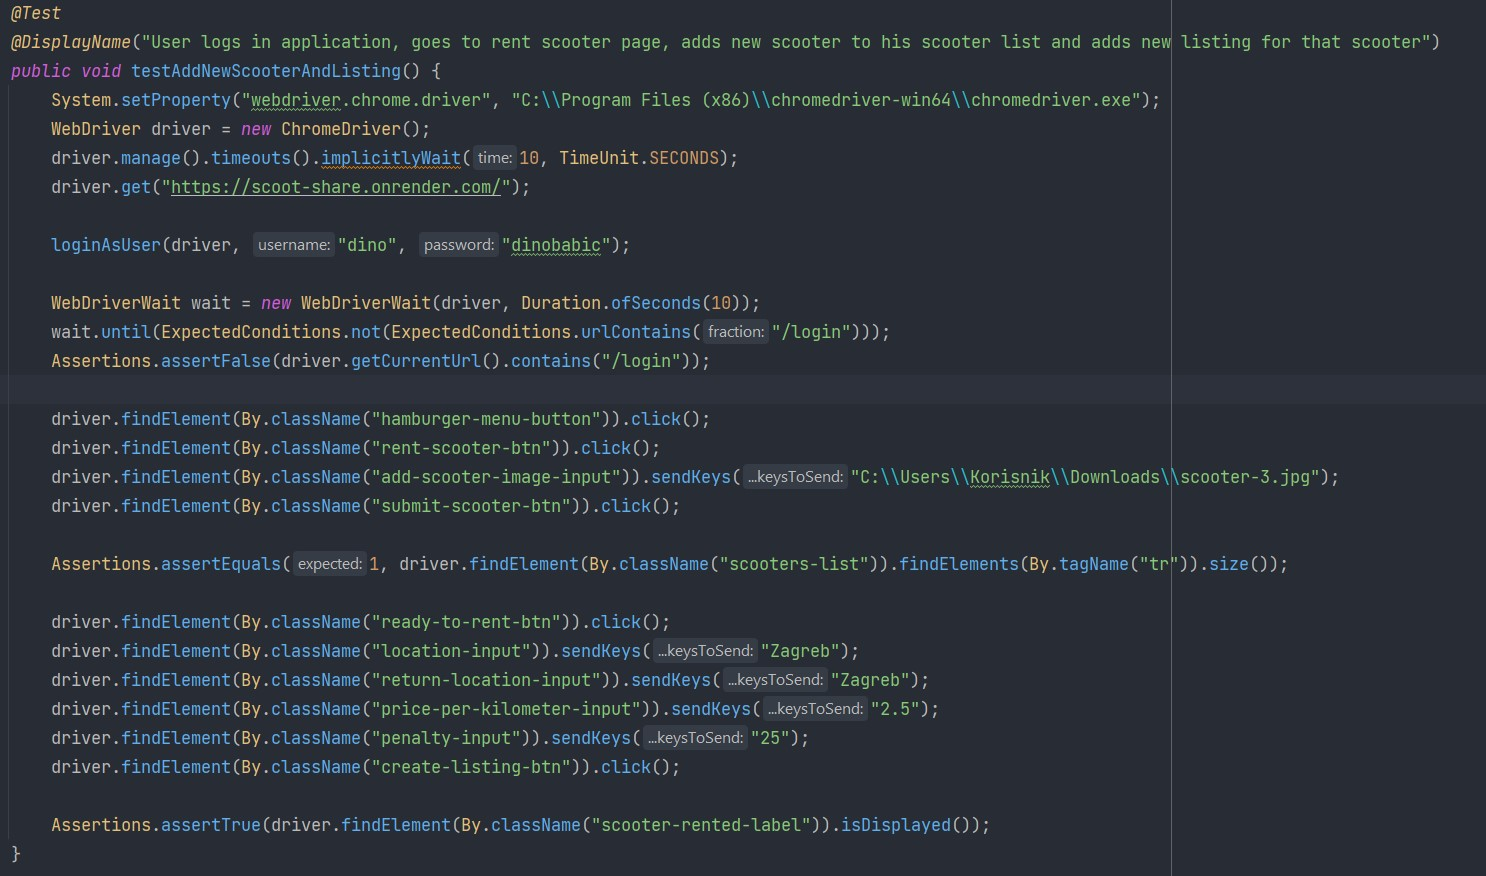
\includegraphics[width=0.6\textwidth]{slike/selenium_test_1.jpg}
			 	\caption{Testiranje dodavanja romobila i oglasa za romobil}
			 	\label{fig:Testiranje dodavanja romobila i oglasa za romobil}
			 \end{figure}
			 
			 \begin{figure}[h]
			 	\centering
			 	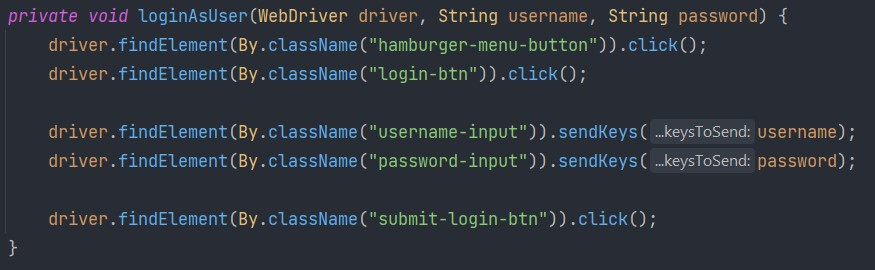
\includegraphics[width=0.6\textwidth]{slike/selenium_login.jpg}
			 	\caption{Funkcija za prijavu korisnika preko objekta tipa WebDriver}
			 	\label{fig:Funkcija za prijavu korisnika preko objekta tipa WebDriver}
			 \end{figure}
			 
			 
			 \indent U sljedećem testu provjerili smo mogućnost unajmljivanja romobila. Prijavili smo se u aplikaciju i odabrali smo prvi oglas na početnoj stranici. Očekivano ponašanje je da nas aplikacija usmjeri na stranicu koja prikazuje detalje o odabrano oglasu te smo to i testirali. Ako je ta provjera uspješno prošla, na stranici smo kliknuli gumb za unajmljivanje romobila. Testirali smo je li nas aplikacija preusmjerila  na stranicu s prikazom trenutno unajmljenih romobila i je li broj trenutno unajmljenih romobila jednak jedan.
			 
			 \begin{figure}[h]
			 	\centering
			 	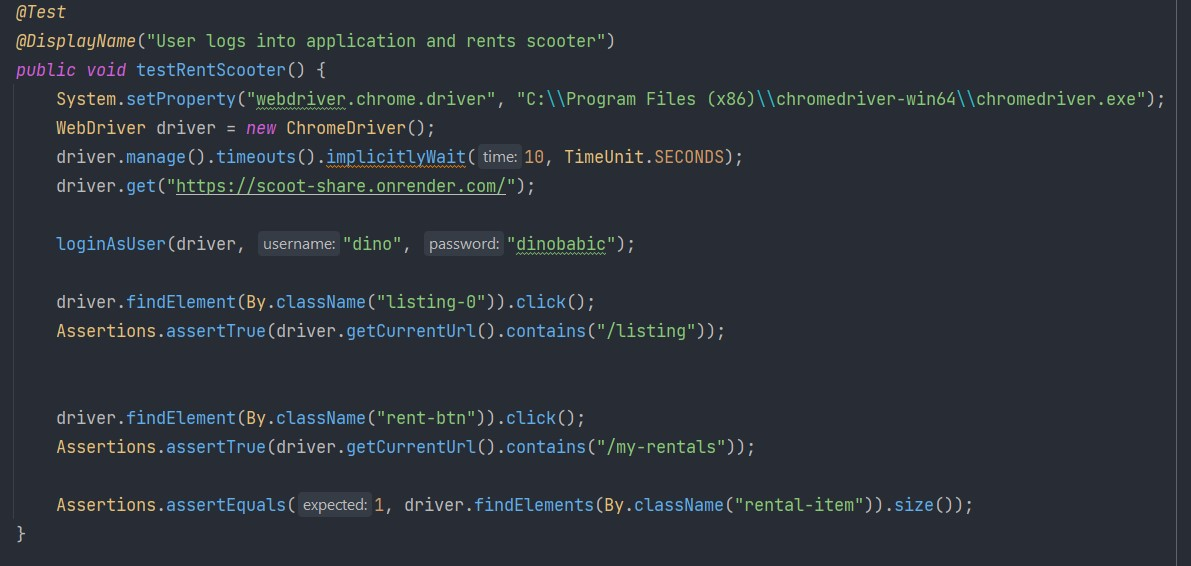
\includegraphics[width=0.7\textwidth]{slike/selenium_test_2.jpg}
			 	\caption{Testiranje unajmljivanja romobila}
			 	\label{fig:Testiranje unajmljivanja romobila}
			 \end{figure}
			 
			 \indent U posljednjem testu provjerili smo funkcionalnost dopisivanja između dva korisnika. Kreirali smo dva objekta tipa WebDriver, jedan za korisnika Dino i jedan za korisnika Marko. Prijavili smo oba korisnika u aplikaciju te smo ih koristeći njihove WebDriver objekte pozicionirali na stranicu za dopisivanje. Testirali smo je li početni broj poruka između ova dva korisnika jednak nuli. Nakon toga korisnik Dino je poslao poruku korisniku Marko. S obzirom na to da je potrebno određeno vrijeme da poruka pristigne do Marka, pozvali smo Thread.sleep(500). Kada se dretva probudila, provjerili smo je li sada broj poruka jednak jedan. Slično smo ponovili još jednom, samo što je sada Marko slao poruku Dini.
			 
			 \begin{figure}
			 	\centering
			 	\subfigure{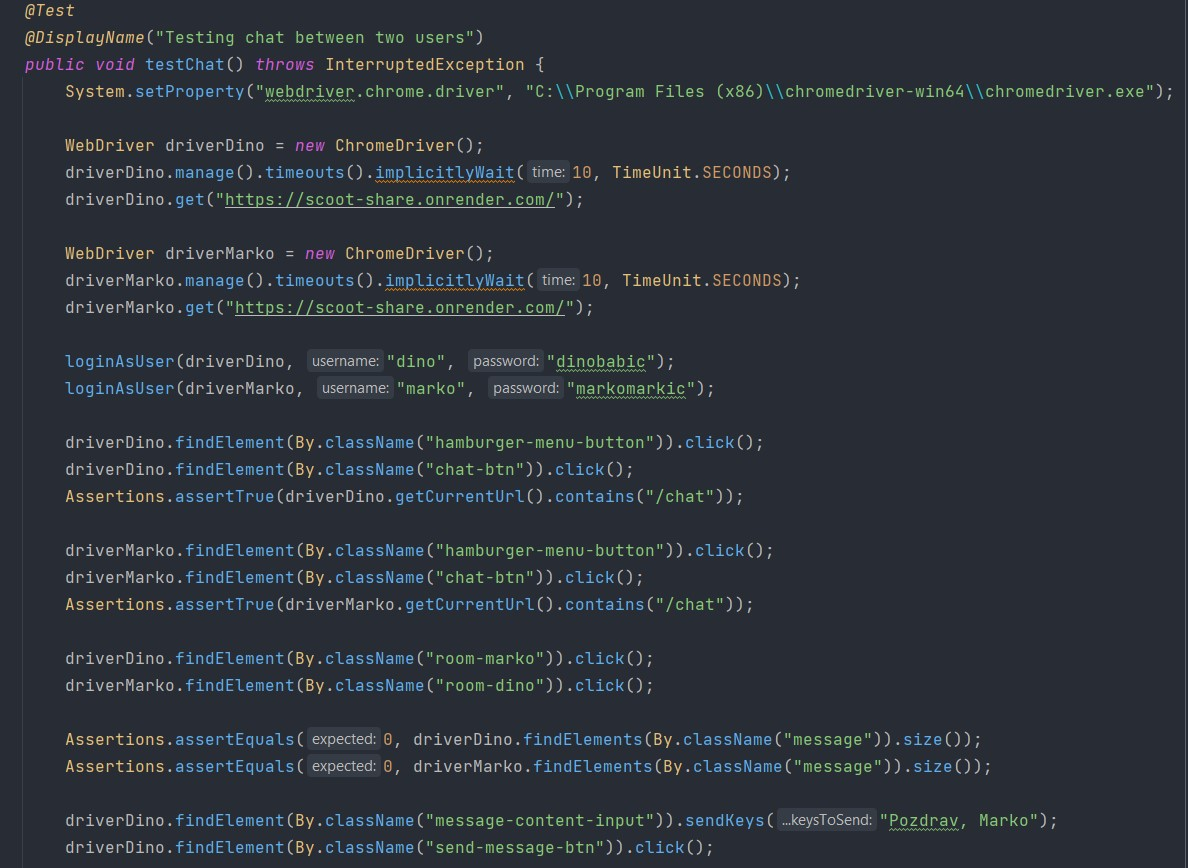
\includegraphics[width=0.7\textwidth]{slike/selenium_test_3_1.jpg}} 
			 	\subfigure{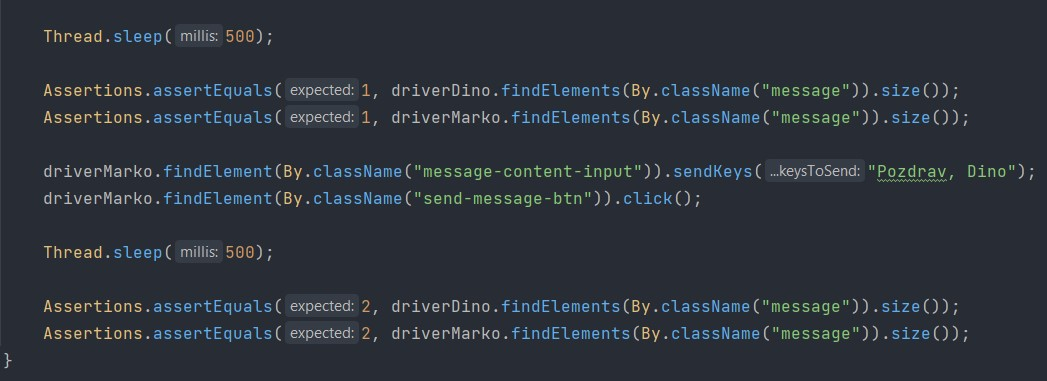
\includegraphics[width=0.7\textwidth]{slike/selenium_test_3_2.jpg}} 
			 	\caption{Testiranje razmjene poruka između korisnika}
			 	\label{fig:Testiranje razmjene poruka između korisnika}
			 \end{figure}
			 
		
		\newpage
		
		\section{Dijagram razmještaja}
			
			 \indent Dijagrami razmještaja opisuju konfiguraciju hardvera i programske podrške korištene u implementaciji sustava unutar njegovog operativnog okruženja. Web poslužitelj i poslužitelj baze podataka smješteni su na poslužiteljskom računalu. Klijenti pristupaju web aplikaciji putem web preglednika. Sustav se temelji na arhitekturi "klijent-poslužitelj", a komunikacija između računala korisnika (iznajmljivača, unajmitelja, administratora) i poslužitelja odvija se putem sigurne HTTPS veze.
			
             \begin{figure}[H]
                \centering
                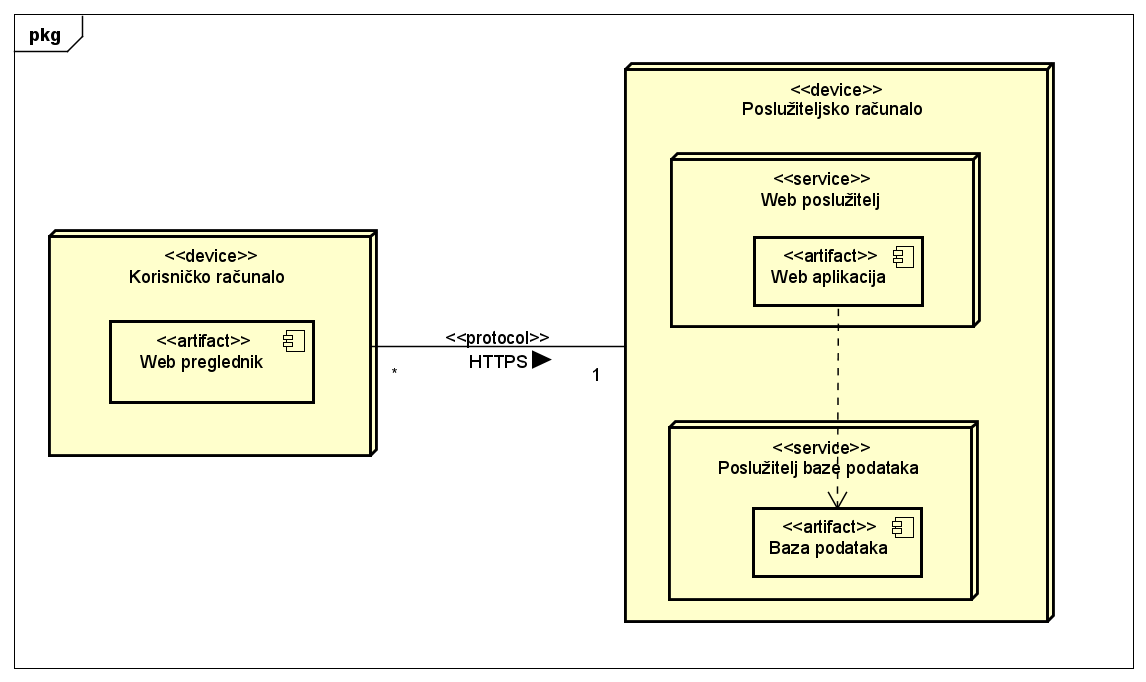
\includegraphics[width=0.8\textwidth]{dijagrami/Dijagram_razmjestaja.png}
				\caption{Dijagram razmještaja}
				\label{fig:your_label}
             \end{figure}

			\eject 
		
		\section{Upute za puštanje u pogon}
		\indent Našu aplikaciju odlučili smo pustit u pogon preko platforme Render. U ovom poglavlju objasnit ćemo korake koje smo proveli kako bi uspješno pustili u pogon aplikaciju.\newline
	
		\textbf{Konfiguracija baze podataka}\newline
		Na web stranici Render potrebno je odabrati izradu nove baze podataka te unijeti željeno ime baze te verziju PostgreSQL-a. Sljedeća slika prikazuje izradu baze podataka.
		\begin{figure}[h]
			\centering
			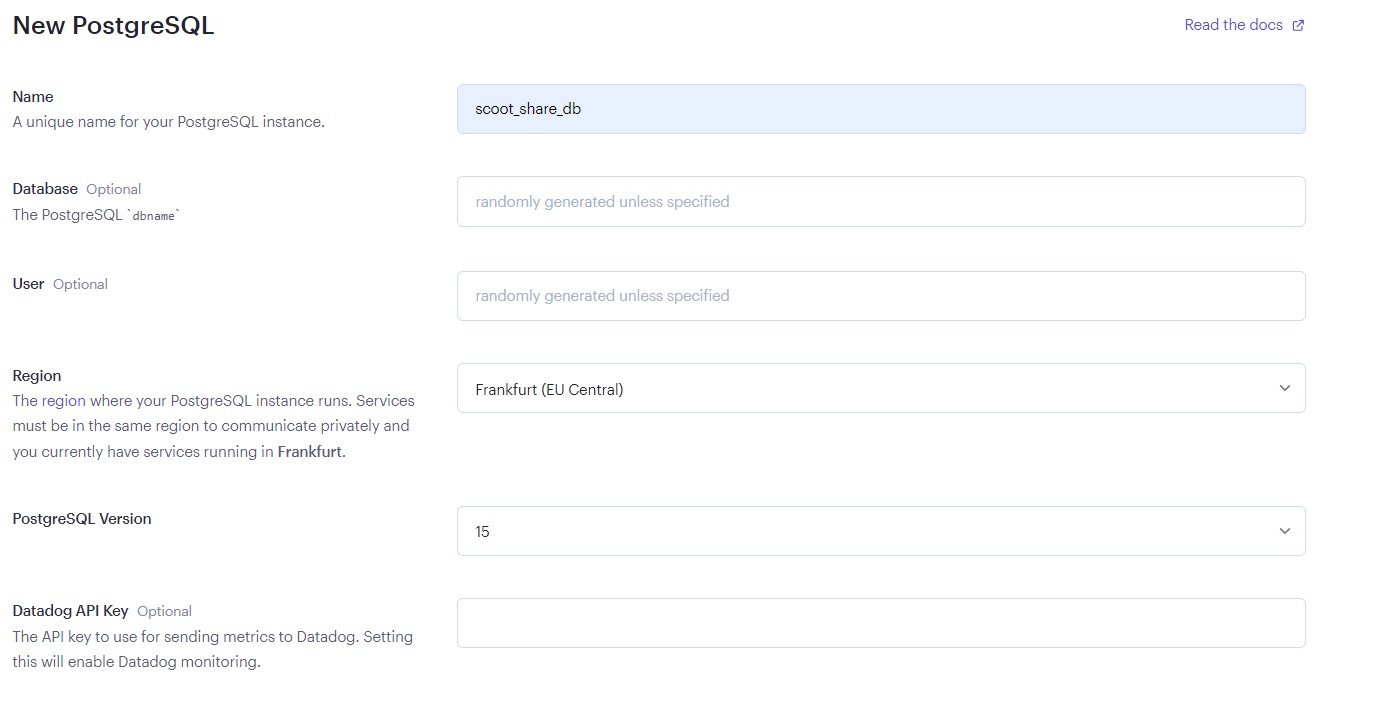
\includegraphics[width=0.8\textwidth]{slike/pustanju_u_pogon_1.jpg}
			\caption{Izrada baze podataka}
			\label{fig:baza podataka}
		\end{figure}
		
		
		\textbf{Konfiguracija backenda}\newline
		Kako bi mogli pustit u pogon našu poslužiteljsku stranu potrebno je učiniti određene izmjene. Potrebno je preurediti application.properties file tako da se dodaju globalne varijable koje će se koristit na Renderu. Također, treba dodati i Dockerfile koji sadrži niz instrukcija za izgradnju Docker kontejnera. 
		
		\begin{figure}
			\centering
			\subfigure{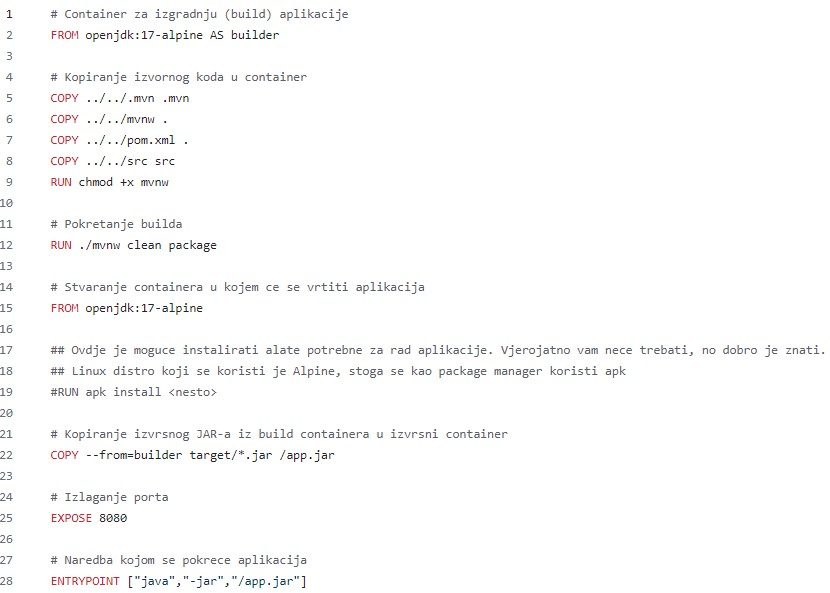
\includegraphics[width=0.24\textwidth]{slike/pustanju_u_pogon_2.jpg}} 
			\subfigure{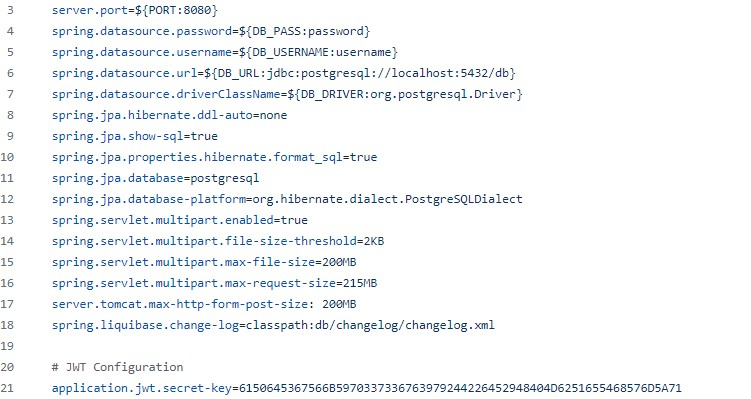
\includegraphics[width=0.24\textwidth]{slike/pustanju_u_pogon_3.jpg}} 
			\caption{Dockerfile i application.properties}
			\label{fig:dockerfile_application.properties}
		\end{figure}
		
		Nakon što je prvi korak odrađen potrebno je konfigurirati backend na Renderu. Odabiremo novi Web Service, nakon toga povežemo naš github repository s Renderom. 
		
		\begin{figure}[h]
			\centering
			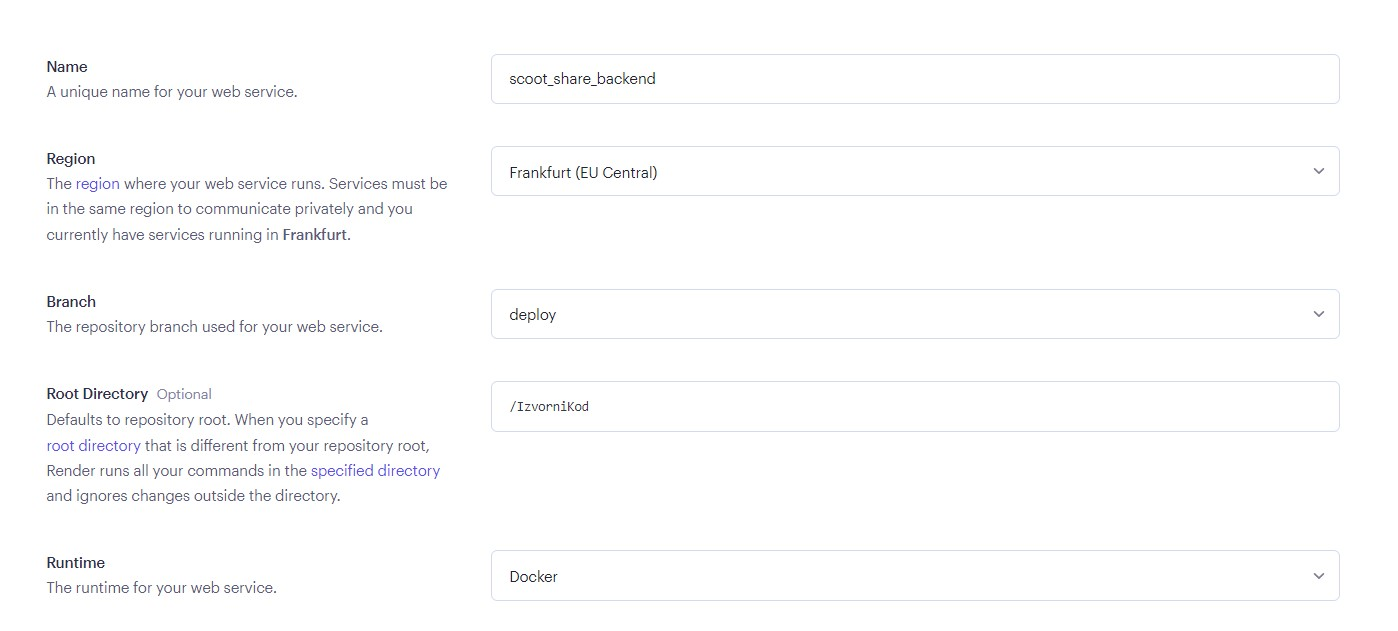
\includegraphics[width=0.8\textwidth]{slike/pustanju_u_pogon_4.jpg}
			\caption{Kreiranje backenda na Renderu}
			\label{fig:backend_render}
		\end{figure}
		
		\textbf{Konfiguracija frontenda}
		Potrebno je u našoj frontend React aplikaciji u datoteci package.json dodati ovisnosti prema http-proxy-middleware, dotenv, express. Zatim treba dodati datoteku /src/setupProxy.js koja služi kao proxy server za lokalni development (redirecta api pozive na localhost:8080), odnosno kad se koristi react-scripts start skripta. Posljednja datoteka koju treba dodati je app.js u kojoj se nalazi express server za produkcijski proxy i posluživanje frontenda. Jednom kada su sve izmjene napravljene i pohranjene u repozitorij kreirajmo Web Servis na Renderu za frontend. 
			
		\begin{figure}[h]
			\centering
			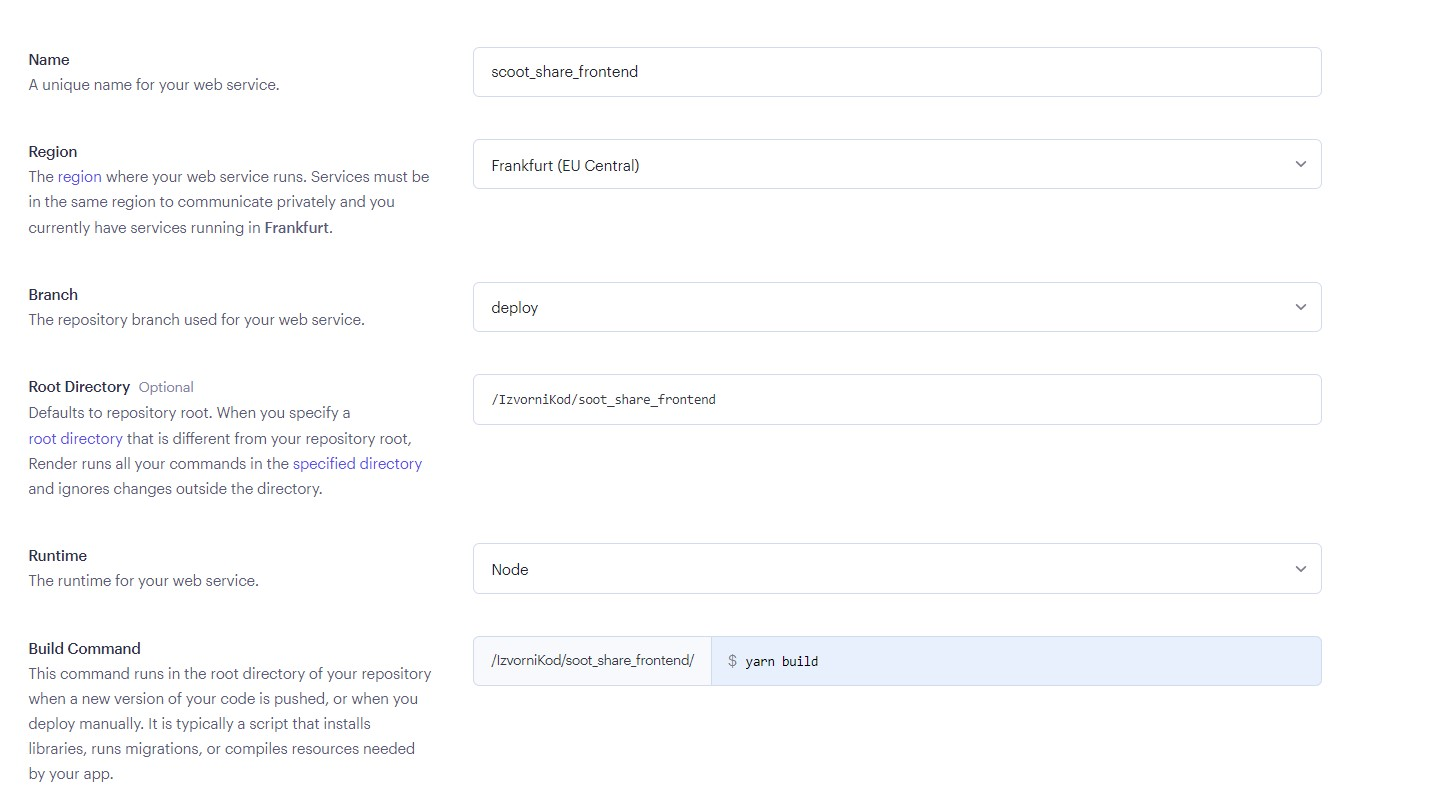
\includegraphics[width=0.8\textwidth]{slike/pustanju_u_pogon_5.jpg}
			\caption{Kreiranje frontenda na Renderu}
			\label{fig:frontend_render}
		\end{figure}
		
		Renderu će trebati jedno vrijeme da pokrene aplikacije te kada završi prikazat će URL adresu preko koje možemo pristupiti našoj aplikaciji. S obzirom na to da Render nudi besplatno puštanje u pogon za očekivat je da će aplikacija raditi sporije, no za naše potrebe je to bilo sasvim dovoljno.